\documentclass[pdflatex,compress]{beamer}

%\usetheme[dark,framenumber,totalframenumber]{ElektroITK}
\usetheme[darktitle,framenumber,totalframenumber]{ElektroITK}
\usepackage{graphicx}
\usepackage{multicol}

\title{Data Communications}

\subtitle{Chapter 2 - Protocol Architecture}

\author{Mifta Nur Farid}

\date{22 February 2023}

\begin{document}

\maketitle

\begin{frame}
	\frametitle{The Need for a Protocol Architecture}
	\begin{itemize}
		\item data exchange can involve complex
		procedures, cf. file transfer example
		\item better if task broken into subtasks
		\item implemented separately in layers in stack
		\begin{itemize}
			\item each layer provides functions needed to
			perform comms for layers above
			\item using functions provided by layers below
		\end{itemize}
		\item peer layers communicate with a protocol
	\end{itemize}
\end{frame}

\begin{frame}
	\frametitle{Key Elements of a Protocol}
	\begin{itemize}
		\item syntax - data format
		\item semantics - control info \& error handling
		\item timing - speed matching \& sequencing
	\end{itemize}
\end{frame}

\begin{frame}
	\frametitle{TCP/IP Protocol Architecture}
	\begin{itemize}
		\item developed by US Defense Advanced Research Project Agency (DARPA)
		\item for ARPANET packet switched network
		\item used by the global Internet
		\item protocol suite comprises a large collection of standardized protocols
	\end{itemize}
\end{frame}

\begin{frame}
	\frametitle{A Simple Protocol Architecture}
	\begin{figure}
		\centering
		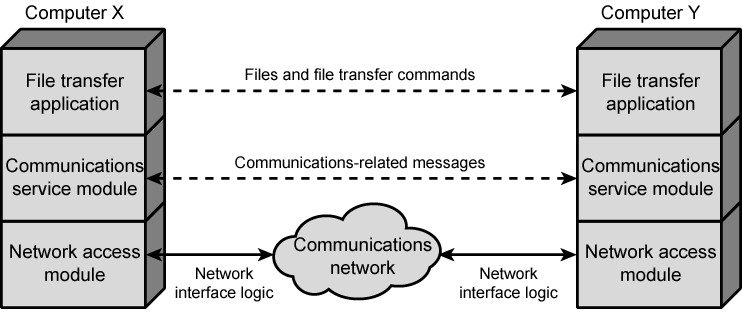
\includegraphics[width=\linewidth]{img/img01}
	\end{figure}
\end{frame}

\begin{frame}
	\frametitle{TCP/IP Layers}
	\begin{itemize}
		\item no official model but a working one
		\begin{itemize}
			\item Application layer
			\item Host-to-host, or transport layer
			\item Internet layer
			\item Network access layer
			\item Physical layer
		\end{itemize}
	\end{itemize}
\end{frame}

\begin{frame}
	\frametitle{Physical Layer}
	\begin{itemize}
		\item concerned with physical interface between computer and network
		\item concerned with issues like:
		\begin{itemize}
			\item characteristics of transmission medium
			\item signal levels
			\item data rates
			\item other related matters
		\end{itemize}
	\end{itemize}
\end{frame}

\begin{frame}
	\frametitle{Network Access Layer}
	\begin{itemize}
		\item exchange of data between an end system and attached network
		\item concerned with issues like:
		\begin{itemize}
			\item destination address provision
			\item invoking specific services like priority
			\item access to \& routing data across a network link between two attached systems
		\end{itemize}
		\item allows layers above to ignore link specifics
	\end{itemize}
\end{frame}

\begin{frame}
	\frametitle{Internet Layer (IP)}
	\begin{itemize}
		\item routing functions across multiple networks
		\item for systems attached to different networks
		\item using IP protocol
		\item implemented in end systems and routers
		\item routers connect two networks and relays data between them
	\end{itemize}
\end{frame}

\begin{frame}
	\frametitle{Transport Layer (TCP)}
	\begin{itemize}
		\item common layer shared by all applications
		\item provides reliable delivery of data
		\item in same order as sent
		\item commonly uses TCP
	\end{itemize}
\end{frame}

\begin{frame}
	\frametitle{Application Layer}
	\begin{itemize}
		\item provide support for user applications
		\item need a separate module for each type of application
	\end{itemize}
\end{frame}

\begin{frame}
	\frametitle{Operation of TCP and IP}
	\begin{figure}
		\centering
		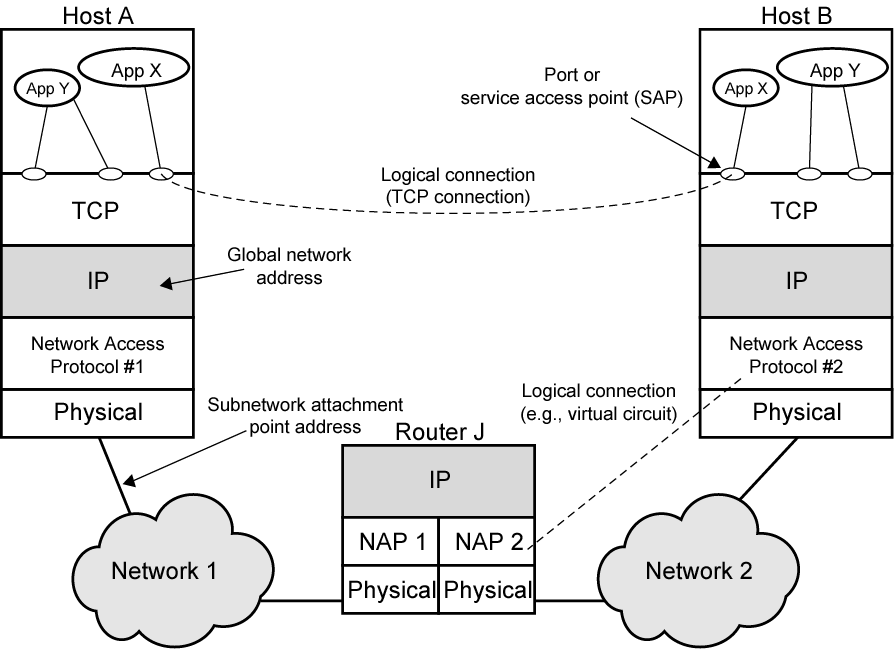
\includegraphics[width=0.8\linewidth]{img/img02}
	\end{figure}
\end{frame}

\begin{frame}
	\frametitle{Addressing Requirements}
	\begin{itemize}
		\item two levels of addressing required
		\item each host on a subnet needs a unique global network address
		\begin{itemize}
			\item its IP address
		\end{itemize}
		\item each application on a (multi-tasking) host needs a unique address within the host
		\begin{itemize}
			\item known as a port
		\end{itemize}
	\end{itemize}
\end{frame}

\begin{frame}
	\frametitle{Operation of TCP and IP}
	\begin{figure}
		\centering
		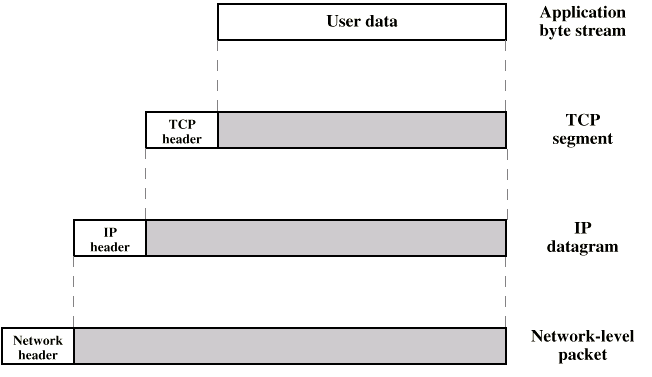
\includegraphics[width=0.8\linewidth]{img/img03}
	\end{figure}
\end{frame}

\begin{frame}
	\frametitle{Transmission Control Protocol (TCP)}
	\begin{itemize}
		\item usual transport layer is (TCP)
		\item provides a reliable connection for transfer of data between applications
		\item a TCP segment is the basic protocol unit
		\item TCP tracks segments between entities for duration of each connection
	\end{itemize}
\end{frame}

\begin{frame}
	\frametitle{TCP Header}
	\begin{figure}
		\centering
		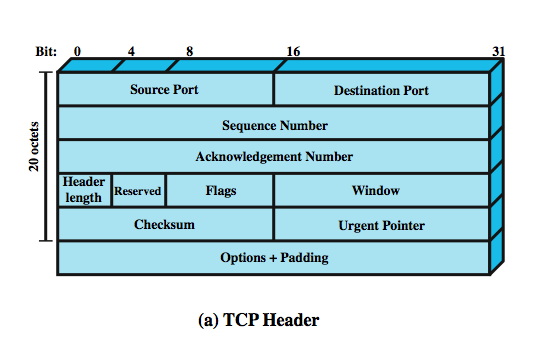
\includegraphics[width=0.8\linewidth]{img/img04}
	\end{figure}
\end{frame}

\begin{frame}
	\frametitle{User Datagram Protocol (UDP)}
	\begin{itemize}
		\item an alternative to TCP
		\item no guaranteed delivery
		\item no preservation of sequence
		\item no protection against duplication
		\item minimum overhead
		\item adds port addressing to IP
	\end{itemize}
\end{frame}

\begin{frame}
	\frametitle{UDP Header}
	\begin{figure}
		\centering
		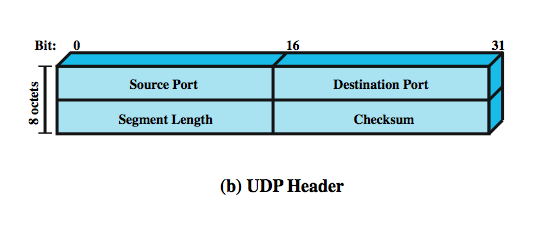
\includegraphics[width=0.8\linewidth]{img/img05}
	\end{figure}
\end{frame}

\begin{frame}
	\frametitle{IP Header}
	\begin{figure}
		\centering
		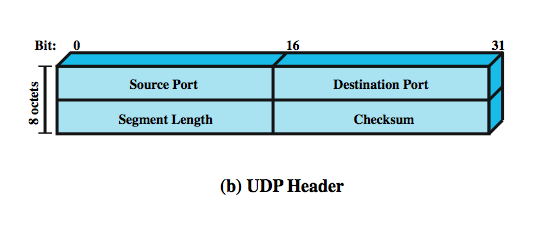
\includegraphics[width=0.8\linewidth]{img/img05}
	\end{figure}
\end{frame}

\begin{frame}
	\frametitle{IPv6 Header}
	\begin{figure}
		\centering
		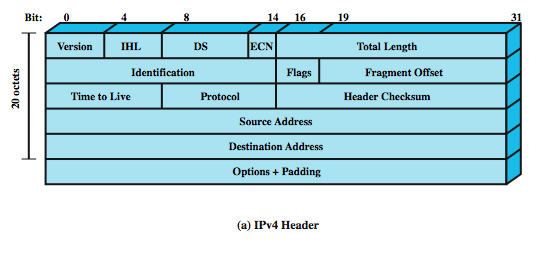
\includegraphics[width=\linewidth]{img/img06}
	\end{figure}
\end{frame}

\begin{frame}
	\frametitle{TCP/IP Applications}
	\begin{itemize}
		\item have a number of standard TCP/IP applications such as
		\begin{itemize}
			\item Simple Mail Transfer Protocol (SMTP)
			\item File Transfer Protocol (FTP)
			\item Telnet
		\end{itemize}
	\end{itemize}
\end{frame}

\begin{frame}
	\frametitle{Some TCP/IP Protocols}
	\begin{figure}
		\centering
		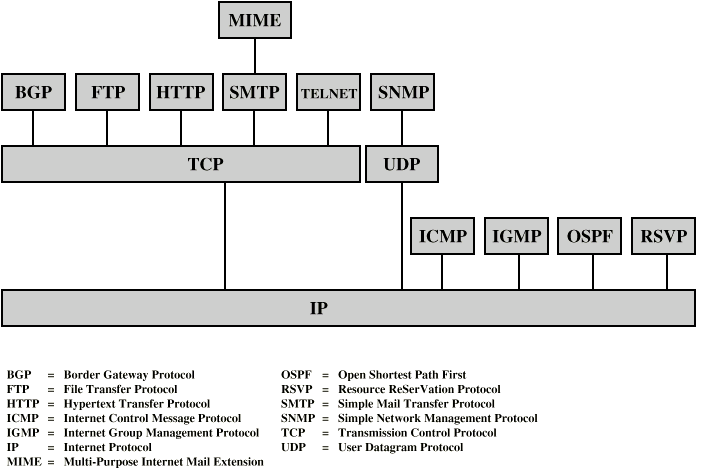
\includegraphics[width=\linewidth]{img/img07}
	\end{figure}
\end{frame}

\begin{frame}
	\frametitle{OSI}
	\begin{itemize}
		\item Open Systems Interconnection
		\item developed by the International Organization for Standardization (ISO)
		\item has seven layers
		\item is a theoretical system delivered too late!
		\item TCP/IP is the de facto standard
	\end{itemize}
\end{frame}

\begin{frame}
	\frametitle{OSI Layers}
	\begin{figure}
		\centering
		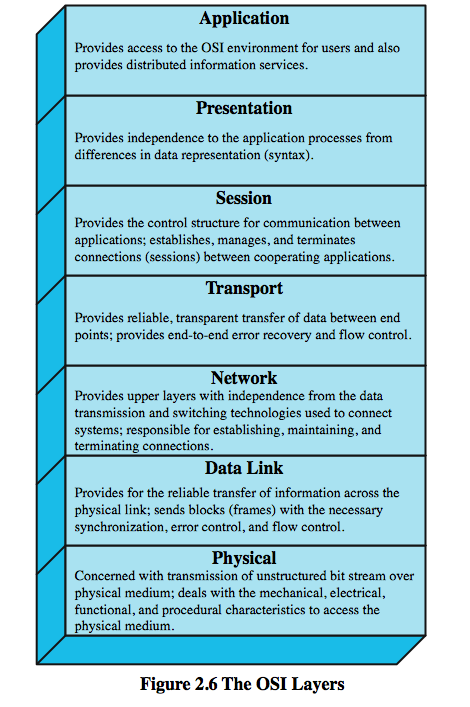
\includegraphics[width=0.6\textheight]{img/img08}
	\end{figure}
\end{frame}

\begin{frame}
	\frametitle{OSI vs TCP/IP}
	\begin{figure}
		\centering
		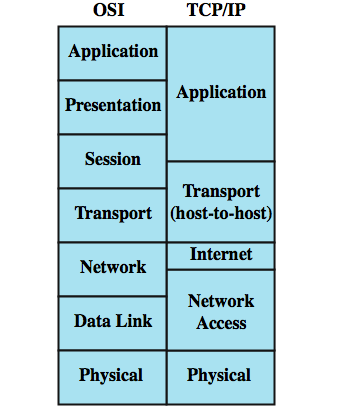
\includegraphics[width=0.6\textheight]{img/img09}
	\end{figure}
\end{frame}

\begin{frame}
	\frametitle{Standardized Protocol Architectures}
	\begin{figure}
		\centering
		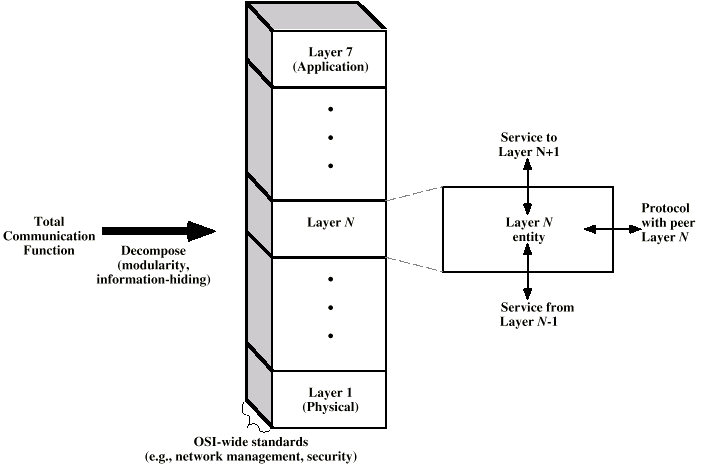
\includegraphics[width=\textheight]{img/img10}
	\end{figure}
\end{frame}

\begin{frame}
	\frametitle{Layer Specific Standards}
	\begin{figure}
		\centering
		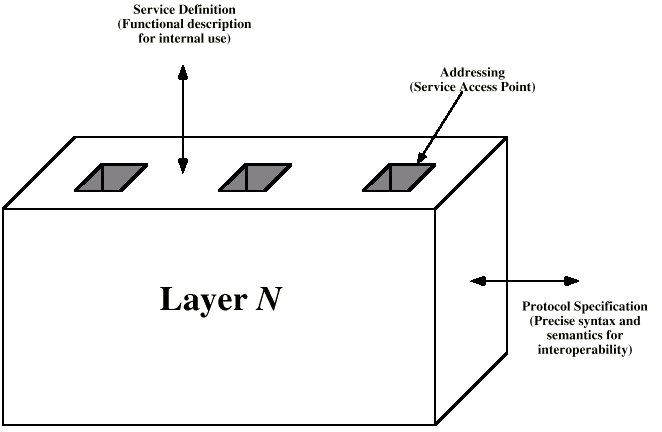
\includegraphics[width=\textheight]{img/img11}
	\end{figure}
\end{frame}

\begin{frame}
	\frametitle{Service Primitives and Parameters}
	\begin{multicols}{2}
		\begin{itemize}
			\item define services between adjacent layers using:
			\item primitives to specify function performed
			\item parameters to pass data and control info
		\end{itemize}
		\columnbreak
		\begin{figure}
			\centering
			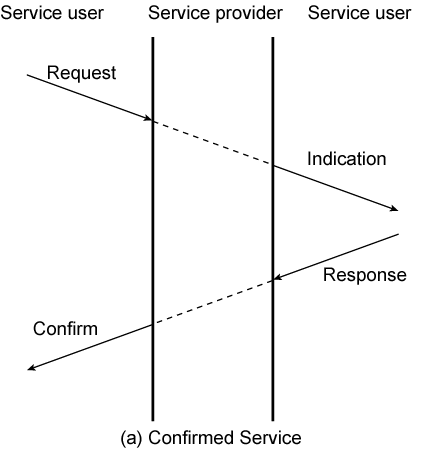
\includegraphics[width=\linewidth]{img/img12}
		\end{figure}
	\end{multicols}
\end{frame}

\begin{frame}
	\frametitle{Primitive Types}
	\begin{itemize}
		\item \textbf{REQUEST}: A primitive issued by a service user to invoke some service and to pass the parameters needed to specify fully the requested service
		\item \textbf{INDICATION}: A primitive issued by a service provider either to: indicate that a procedure has been invoked by the peer service user on the connection and to provide the associated parameters, or notify the service user of a provider-initiated action
		\item \textbf{RESPONSE}: A primitive issued by a service user to acknowledge or complete some procedure previously invoked by an indication to that user
		\item \textbf{CONFIRM}: A primitive issued by a service provider to acknowledge or complete some procedure previously invoked by a request by the service user
	\end{itemize}
\end{frame}

\begin{frame}
	\frametitle{Traditional vs Multimedia Applications}
	\begin{itemize}
		\item traditionally Internet dominated by info retrieval applications
		\begin{itemize}
			\item typically using text and image transfer
			\item eg. email, file transfer, web
		\end{itemize}
		\item see increasing growth in multimedia applications
		\begin{itemize}
			\item involving massive amounts of data
			\item such as streaming audio and video
		\end{itemize}
	\end{itemize}
\end{frame}

\begin{frame}
	\frametitle{Elastic and Inelastic Traffic}
	\begin{itemize}
		\item elastic traffic
		\begin{itemize}
			\item can adjust to delay \& throughput changes over a wide range
			\item eg. traditional “data” style TCP/IP traffic
			\item some applications more sensitive though
		\end{itemize}
		\item inelastic traffic
		\begin{itemize}
			\item does not adapt to such changes
			\item eg. “real-time” voice \& video traffic
			\item need minimum requirements on net arch
		\end{itemize}
	\end{itemize}
\end{frame}

\begin{frame}
	\frametitle{Multimedia Technologies}
	\begin{figure}
		\centering
		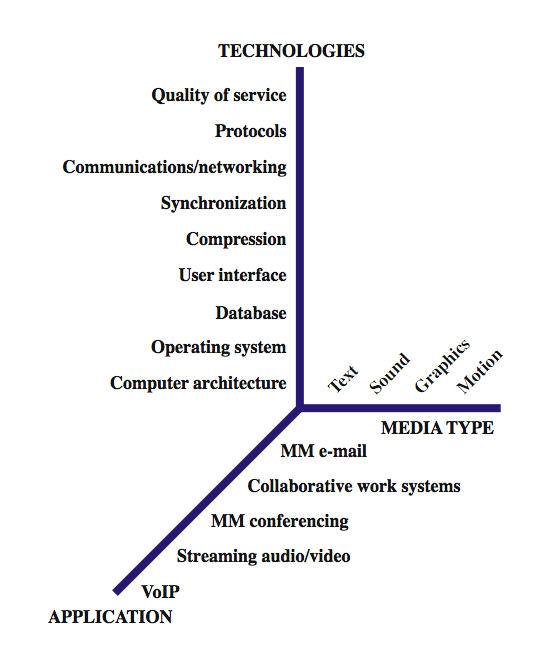
\includegraphics[height=0.9\textheight]{img/img13}
	\end{figure}
\end{frame}

\begin{frame}
	\frametitle{Summary}
	\begin{itemize}
		\item introduced need for protocol architecture
		\item TCP/IP protocol architecture
		\item OSI Model \& protocol architecture standardization
		\item traditional vs multimedia application needs
	\end{itemize}
\end{frame}

\end{document}
